\documentclass[12pt]{article}
\usepackage[utf8]{inputenc}

\title{Lab 6}
\author{Benny Chen - Avaneesh Sathish}
\date{\today}

\usepackage{color}
\usepackage{amsthm}
\usepackage{amssymb} 
\usepackage{amsmath}
\usepackage{listings}
\usepackage{xcolor}
\usepackage{listings}
\usepackage{graphicx}
\usepackage{subcaption}
\usepackage{caption}
\usepackage{tikz}
\usepackage{pgfplots}
\usepackage{pgfplotstable}
\usepackage[hidelinks]{hyperref}

\begin{document}
\maketitle

\section*{Question 1}

\begin{center}
    \includegraphics[scale=.07]{images/q1.jpg}
\end{center}

The Pineapple AP has a dashboard for multiple items of tasks that it could do.
On the dashboard itself it has "cards" that show the statuses of
CPU and RAM, Disk Usage, and Network Data like clients and landscape.
On the left side of the dashboard it has a list of all the tasks that
the AP can do, such as campaigns, PineAP, Recon, Documentation, Modules, and Settings.

\section*{Question 2}

\begin{center}
    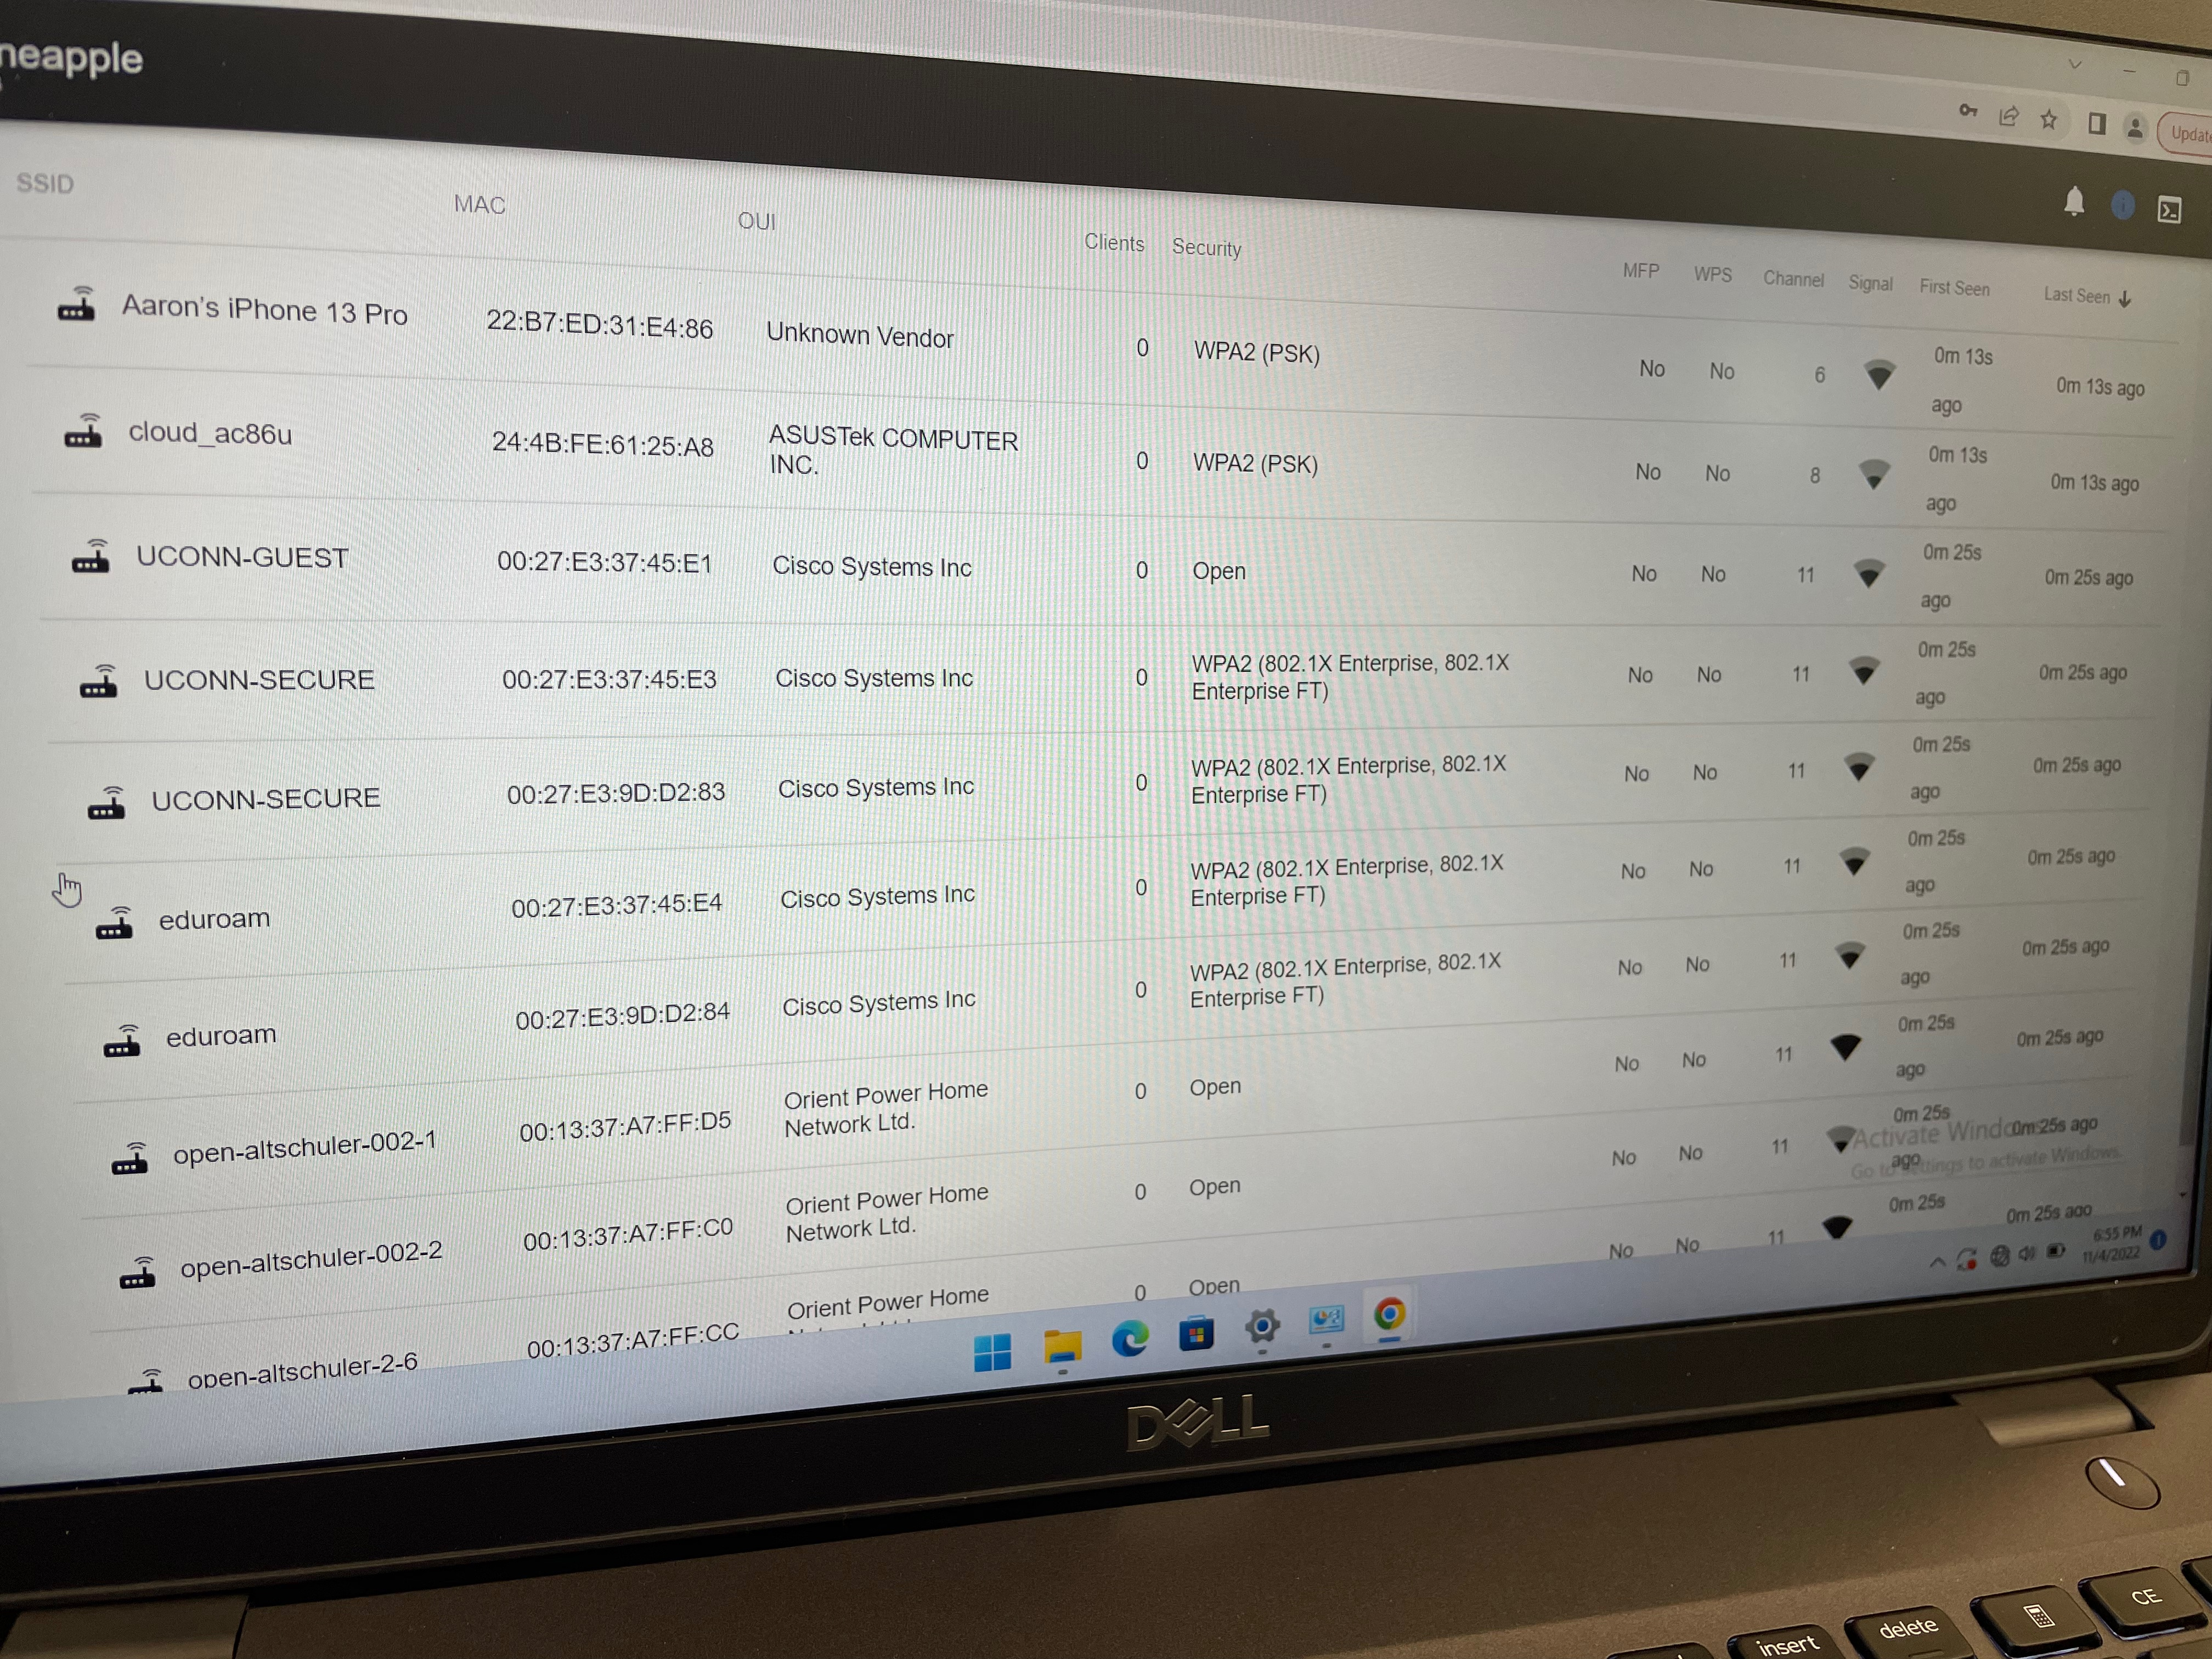
\includegraphics[scale=.07]{images/q2scan_1.jpg}
    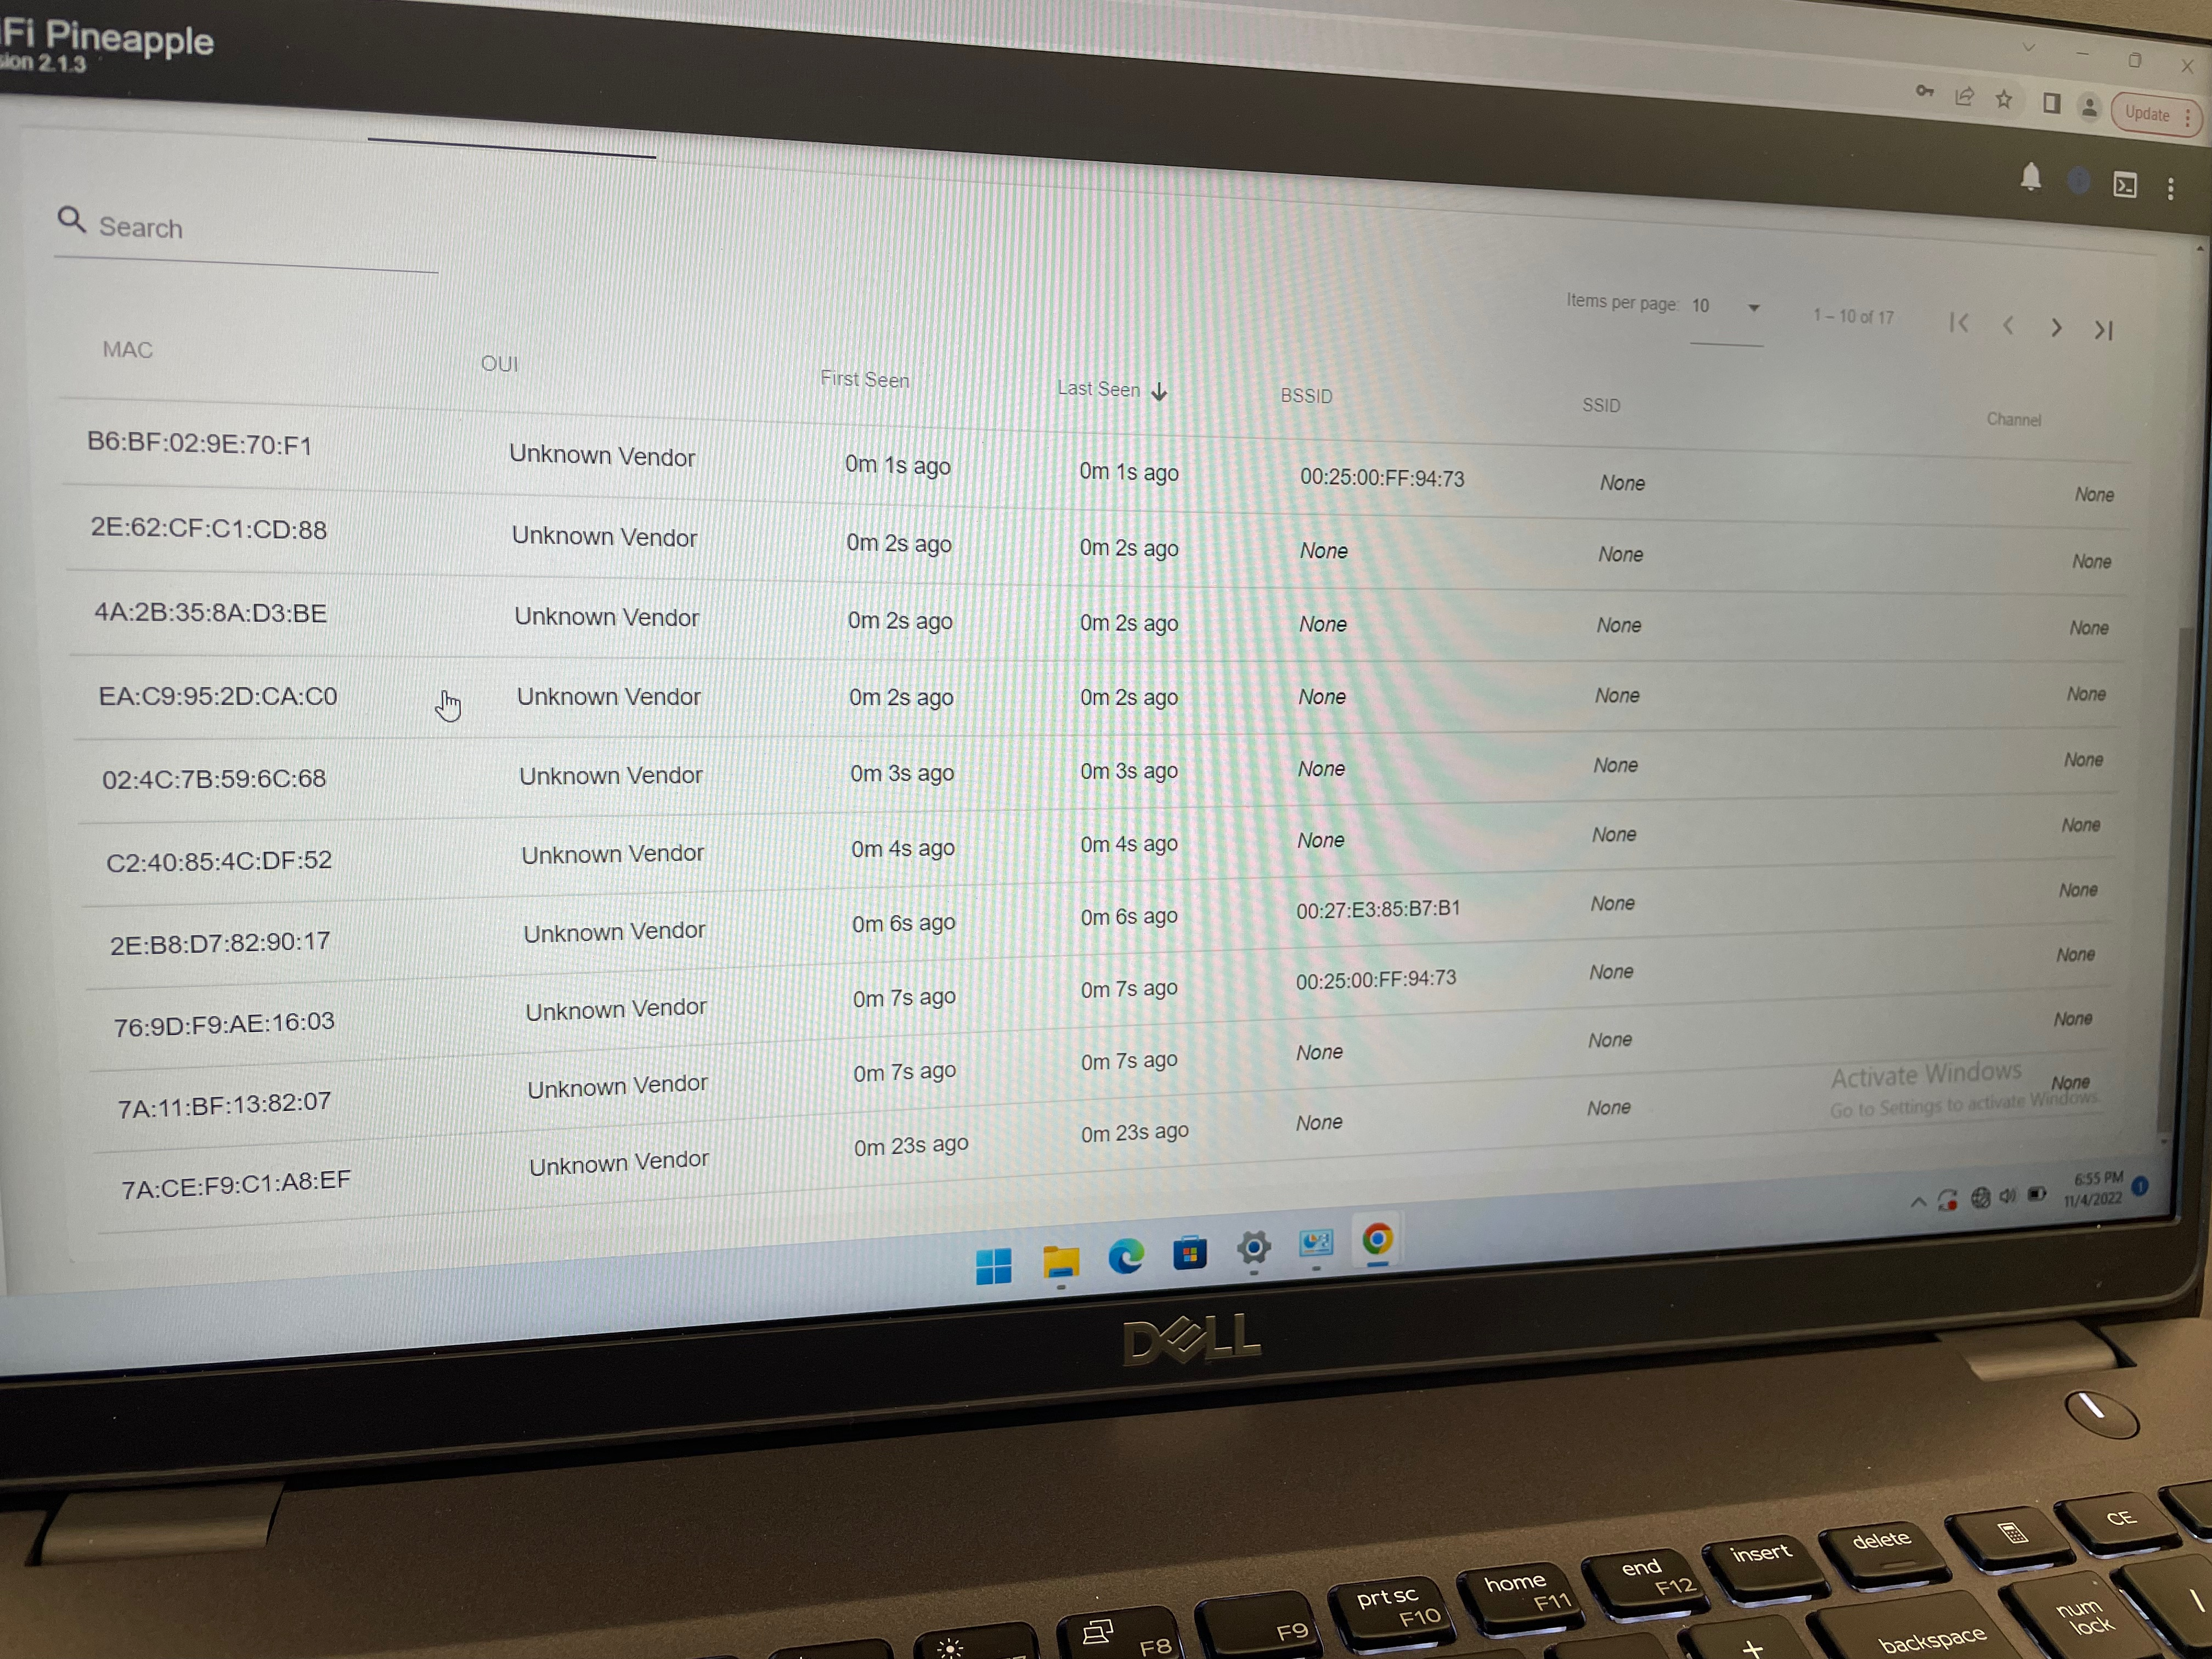
\includegraphics[scale=.07]{images/q2scan_2.jpg}
    \includegraphics[scale=.07]{images/q2_handshake.jpg}
\end{center}

From my understanding, Recon shows all networks and clients in the area while 
Handshakes show the networks and clients that joined. In the recon tab,
it shows the amount of clients and networks in the area along with graphs and charts of them.

\section*{Question 3}

\begin{center}
    \includegraphics[scale=.07]{images/q3_scan1.jpg}
    \includegraphics[scale=.07]{images/q3_handshake.jpg}
\end{center}

\begin{enumerate}
    \item Yes I can see the personal wifi network I created.
    \item Yes I can see all users connected to the network.
    \item CSE 3140 was using WPA2 Enterprise (CCMP) security.
    \item There are a total of 8 columns in the table which are 
    SSID (Network Name), MAC (MAC Address or that devices unique identifier), 
    OUI (Organizationally Unique Identifier for the manufacturer of the device),
    Security (The type of security the network is using), WPS (Whether or not the network is using WPS),
    Channel (The channel the network is using), Signal (The signal strength of the network),
    and Last Seen (The last time the device was seen).
\end{enumerate}

\section*{Question 4}
\begin{center}
    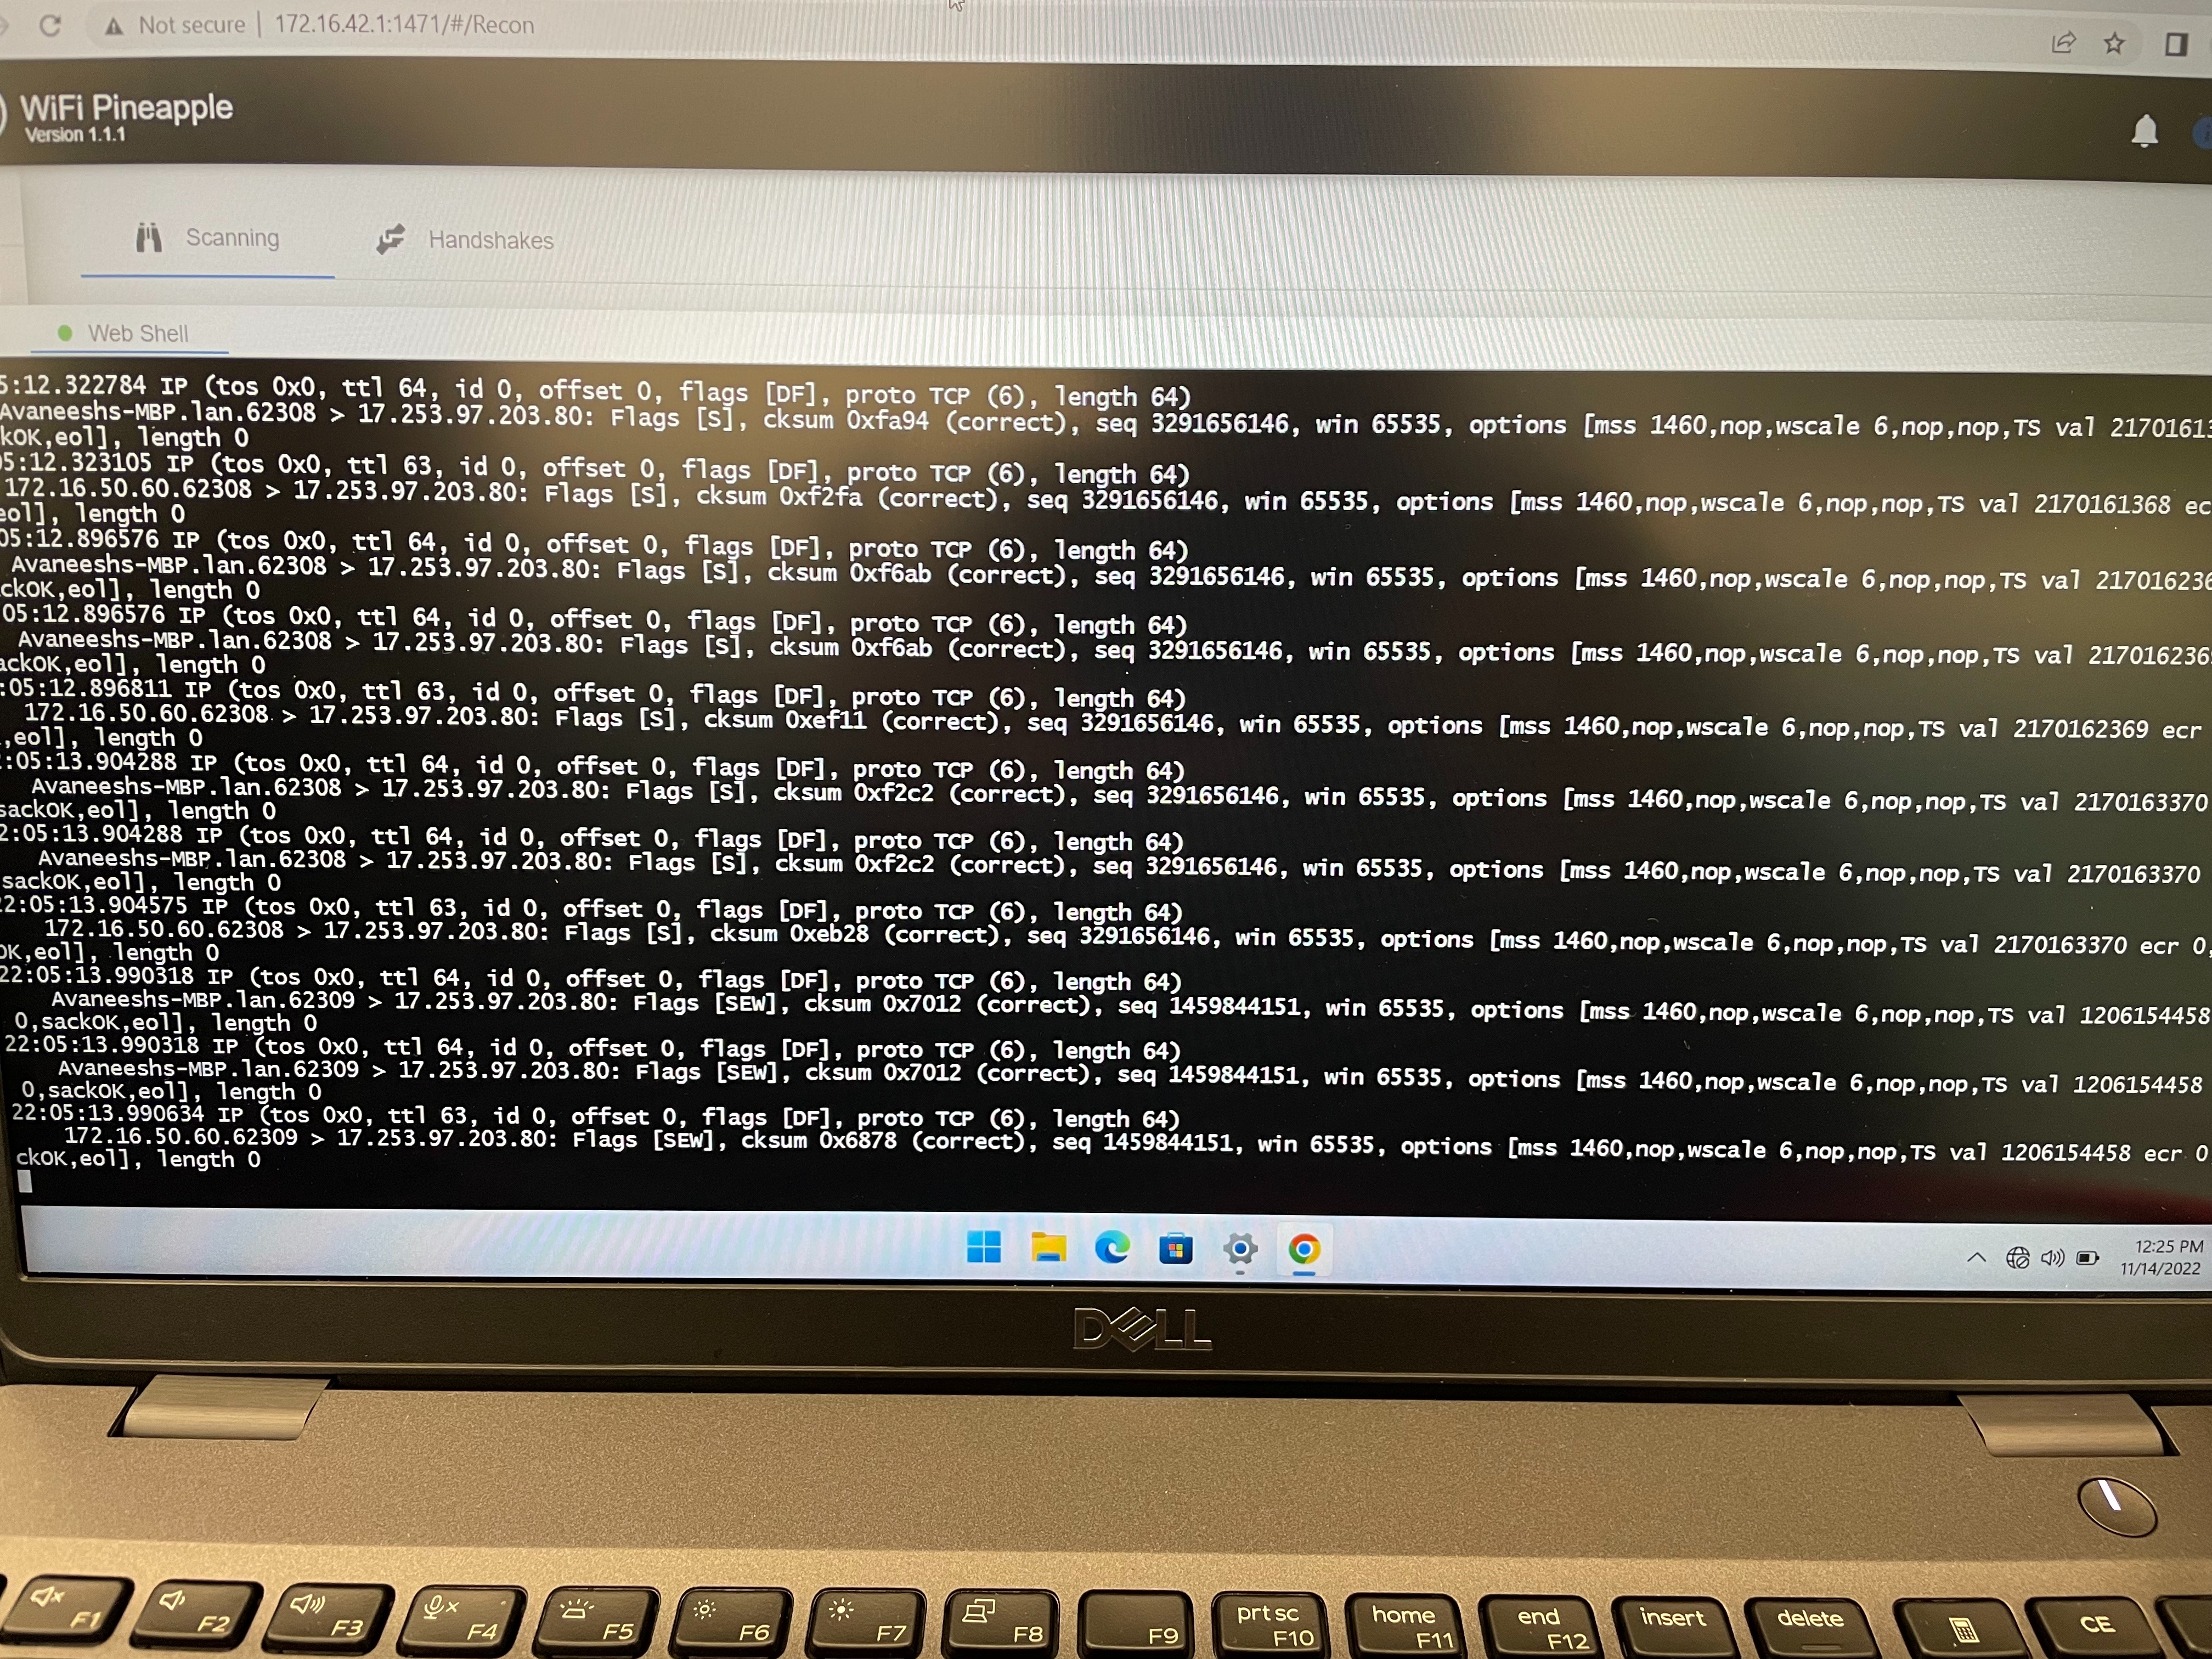
\includegraphics[scale=.07]{images/q4.jpg}
\end{center}

Yes I see traffic, mainly from the connected laptop on the network.
The device is named Avaneeshs-MBP and is being directed to 
17.253.97.203.80. This cooresponds to the IP address of the Pineapple AP.

\section*{Question 5}
\begin{center}
    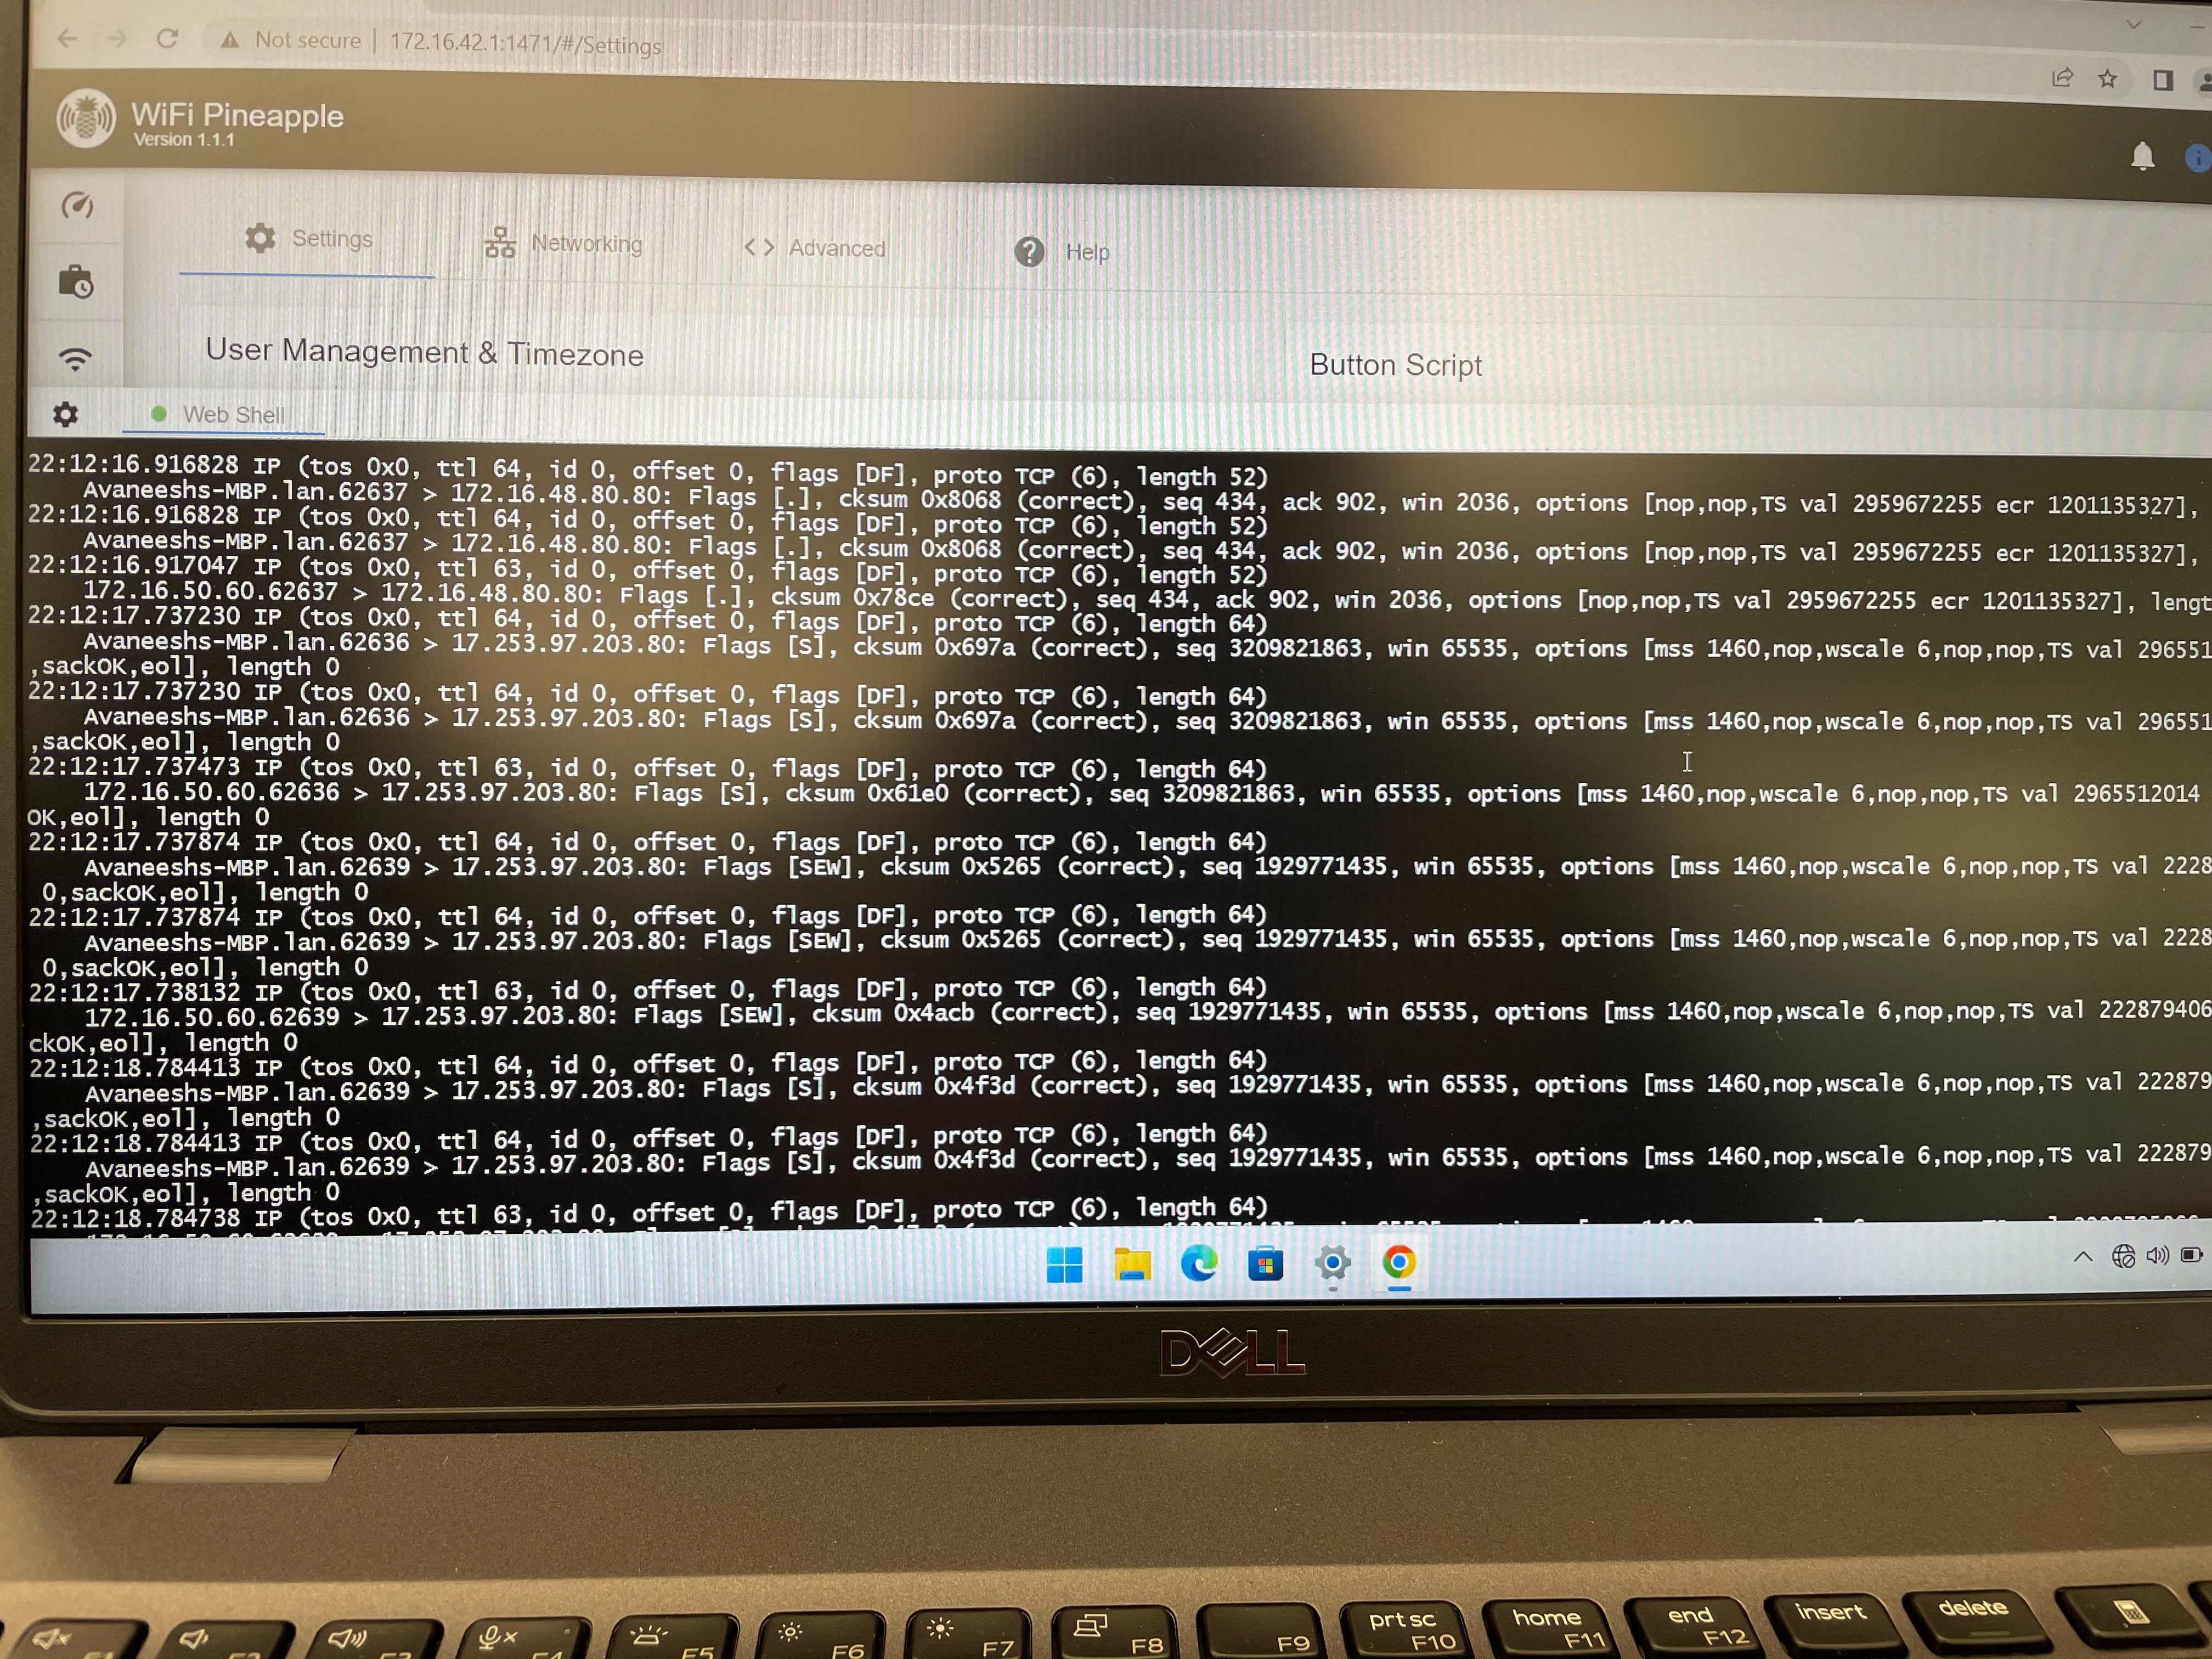
\includegraphics[scale=.07]{images/q5.jpg}
\end{center}

\begin{enumerate}
    \item Yes I can see the traffic from the connected laptop still.
    \item No being on the protected network does not help.
    \item This is because the secure network is still using the Pineapple AP as a router.
\end{enumerate}

\section*{Question 6}

\begin{enumerate}
    \item It seems like non hidden networks are visible. Those with a unknown OUI and SSID cannot have information extracted from them.
    Any open or protected network can be seen.
    \item Yes, UCONN-SECURE is an access point that announces more than one network. There are multiple SSIDs that are UCONN-SECURE but they have different MAC addresses.
    \item The security column lists the type of security the network is using. It can be WPA2, WPA, WEP, or Open, meaning security is being used or not.
\end{enumerate}

\section*{Question 7}

\begin{center}
    \includegraphics[scale=.07]{images/q7.jpg}
\end{center}

Yes I see traffic.

\section*{Question 8}

We could not successfully deauthenticate ourselves from the network. There
were too many clients and networks in the area which interfered with our
network making it unsuccessful. The TA said that this was okay and to just
move on.

\section*{Question 9}

In this question we created DNS entries to redirect the user to a fake
bank website. 


\end{document}